% !TeX spellcheck = ru_RU
% !TeX encoding = UTF-8
\chapter{Конформационное поведение бицикло[3.3.1]нонанов и их аналогов}\label{ch:Conformation:331}


\begin{figure}
\caption{Конформационное поведение аналогов бицикло[3.3.1]нонана}\label{fig:Conformational:Behavior:331:XYZ}
  \centerfloat{
    \begin{tabu} to \textwidth {|X[c]|X[c]|X[c]|}
      \toprule
      \BC{} & \CC{} & \CB{} \\
      \midrule
      \multicolumn{3}{c}{
      \schemestart
      %\ChemPicture
      \chemfig{X?[a]<[:-30,1.25]-[:+30,,,,line width=\boldbondwidth](-[:+45,0.75,,,line width=\boldbondwidth]R')(>[:+120]Z-[:-120](-[:+135,0.75]R)(-[:-150]?[a])(-[:-30]-[:-60]Y?[b]))-[:-+30,,,,line width=\boldbondwidth]?[b,{<}]
      }
      %\ChemPicture
      \arrow{<=>}
      % \ChemPicture
      \chemfig{X?[a]<[:+60]-[:+30,,,,line width=\boldbondwidth](-[:+45,0.75,,,line width=\boldbondwidth]R')(>[:+120]Z-[:-120](-[:+135,0.75]R)(-[:-150]?[a])(-[:-30]-[:-60]Y?[b]))-[:-+30,,,,line width=\boldbondwidth]?[b,{<}]} % 
      \arrow{<=>}
      %\ChemPicture
      \chemfig{X?[a]<[:+60]-[:+30,,,,line width=\boldbondwidth](-[:+45,0.75,,,line width=\boldbondwidth]R')(>[:+120]Z-[:-120](-[:+135,0.75]R)(-[:-150]?[a])(-[:-30]-[:+30,1.25]Y?[b]))-[:-+30,,,,line width=\boldbondwidth]?[b,{<}]}
      \schemestop
      } 
    \\
    \midrule
    \multicolumn{3}{c}{
      \schemestart
      %\ChemPicture
      \chemfig{X?[a]<[:-30,1.25]-[:+30,,,,line width=\boldbondwidth]N(>[:+120]-[:-120](-[:+135,0.75]R)(-[:-150]?[a])(-[:-30]-[:-60]Y?[b]))-[:-+30,,,,line width=\boldbondwidth]?[b,{<}]
      }
      %\ChemPicture
      \arrow{<=>}
      % \ChemPicture
      \chemfig{X?[a]<[:+60]-[:+30,,,,line width=\boldbondwidth]N(>[:+120]-[:-120](-[:+135,0.75]R)(-[:-150]?[a])(-[:-30]-[:-60]Y?[b]))-[:-+30,,,,line width=\boldbondwidth]?[b,{<}]} % 
      \arrow{<=>}
      %\ChemPicture
      \chemfig{X?[a]<[:+60]-[:+30,,,,line width=\boldbondwidth]N(>[:+120]-[:-120](-[:+135,0.75]R)(-[:-150]?[a])(-[:-30]-[:+30,1.25]Y?[b]))-[:-+30,,,,line width=\boldbondwidth]?[b,{<}]}
      \schemestop
    } 
    \\      \midrule
    \multicolumn{3}{c}{
      \schemestart
      %\ChemPicture
      \chemfig{X?[a]<[:-30,1.25]-[:+30,,,,line width=\boldbondwidth]N(>[:+120]-[:-120]N(-[:-150]?[a])(-[:-30]-[:-60]Y?[b]))-[:-+30,,,,line width=\boldbondwidth]?[b,{<}]
      }
      %\ChemPicture
      \arrow{<=>}
      % \ChemPicture
      \chemfig{X?[a]<[:+60]-[:+30,,,,line width=\boldbondwidth]N(>[:+120]-[:-120]N(-[:-150]?[a])(-[:-30]-[:-60]Y?[b]))-[:-+30,,,,line width=\boldbondwidth]?[b,{<}]} % 
      \arrow{<=>}
      %\ChemPicture
      \chemfig{X?[a]<[:+60]-[:+30,,,,line width=\boldbondwidth]N(>[:+120]-[:-120]N(-[:-150]?[a])(-[:-30]-[:+30,1.25]Y?[b]))-[:-+30,,,,line width=\boldbondwidth]?[b,{<}]}
      \schemestop
    } 
    \\ \bottomrule
    \end{tabu}
  }
\end{figure}



\section{Конформационые энергии, эффекты и строение конформеров}

Корреляционные диаграммы конформационной энергии аналогов бицикло[3.3.1]нонана\dots~\cite{Pisarev:2019}

Применение QTAIM к анализу~\cite{Bushmarinov:UX:2009,Bushmarinov:2011}

\newcommand{\ScaleCorrStr}{0.55}

\begin{figure*}
  \caption{Диаграмма корреляции конформационной энергии для некоторых вариантов симметричного гетероаналогичного замещения в бицикло[3.3.1]нонане (MP4(2) / aug-cc-pVDZ,~ккал/моль)~\cite{Pisarev:2013:rus,Pisarev:2013}}\label{fig:Conform331:MP2}
  \centering
  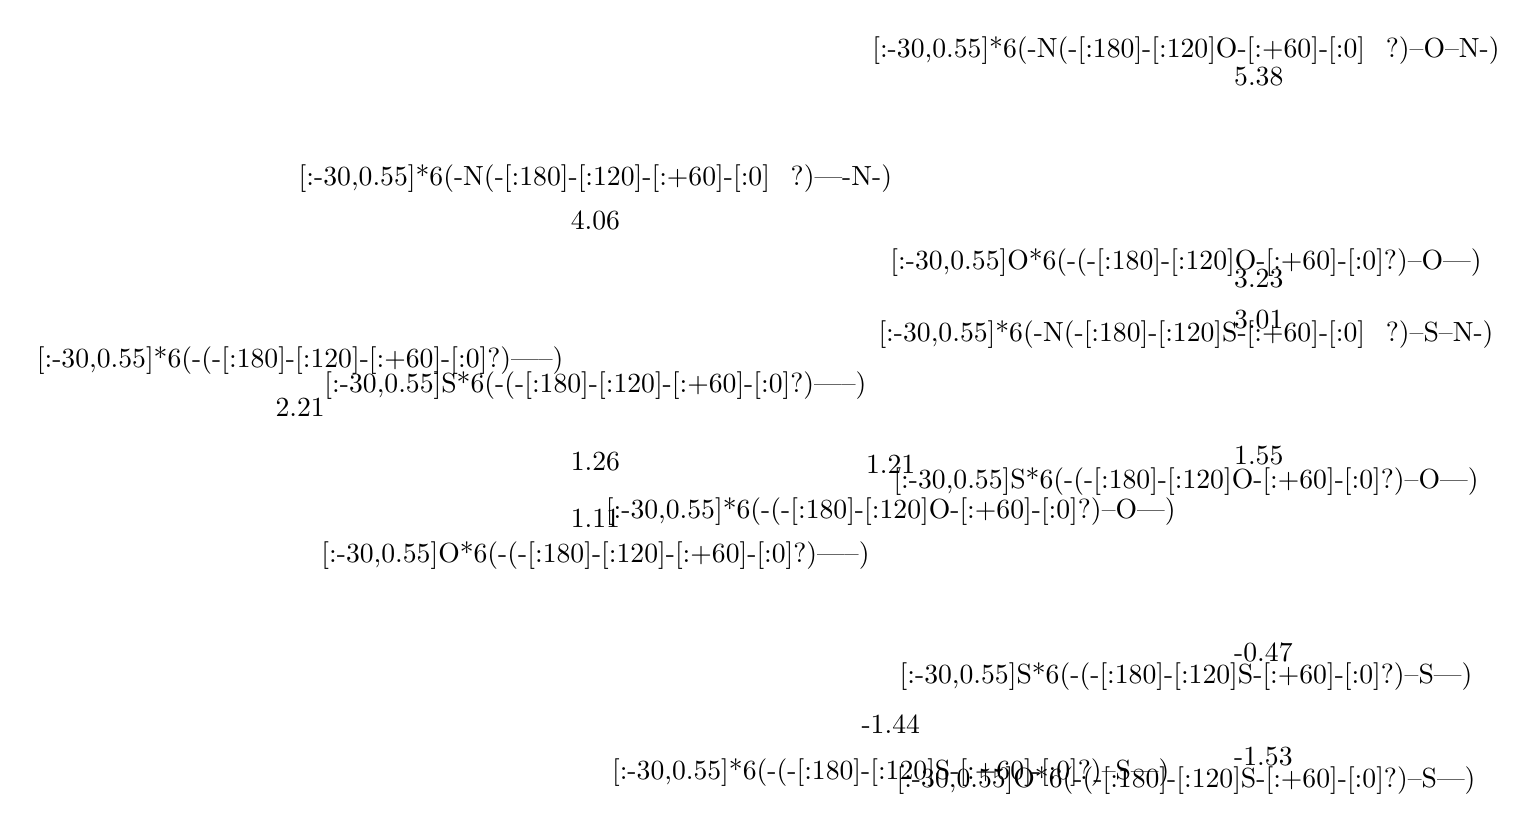
\begin{tikzpicture}[xscale=3.75,yscale=1.25] %
    \DrawCorrFrame{-2}{6};
%
    % [O x 2O]
    \begin{scope}[red,dashed]
      \DrawQuadCorrelation{2.21}{1.11}{1.21}{3.23}
    \end{scope}
    % [O x 2S]
    \begin{scope}[red,dotted]
      \DrawQuadCorrelation{2.21}{1.11}{-1.44}{-1.53}
    \end{scope}
    % [S x 2O]
    \begin{scope}[black,dashed]
      \DrawQuadCorrelation{2.21}{1.26}{1.21}{1.55}
    \end{scope}
    % [S x 2S]
    \begin{scope}[black,dotted]
      \DrawQuadCorrelation{2.21}{1.26}{-1.44}{-0.47}
    \end{scope}
    % [2N x 2O]
    \begin{scope}[blue,dashed]
      \DrawQuadCorrelation{2.21}{4.06}{1.21}{5.38}
    \end{scope}
    % [2N x 2S]
    \begin{scope}[blue,dotted]
      \DrawQuadCorrelation{2.21}{4.06}{-1.44}{3.01}
    \end{scope}
    %structures:
    % bicyclo[3.3.1]nonane
\draw(1.0, 2.25) node [anchor=south] {\chemfig{[:-30,\ScaleCorrStr]*6(-(-[:180]-[:120]-[:+60]-[:0]?)-----)}};
    \draw(1.0, 2.20) node [anchor=north] {\num{2.21}};
    %
1-azabicyclo[3.3.1]nonane
\draw(2.0, 4.10) node [anchor=south] {\chemfig{[:-30,\ScaleCorrStr]*6(-N(-[:180]-[:120]-[:+60]-[:0]\phantom{N}?)----N-)}};
    \draw(2.0, 4.10) node [anchor=north] {\num{4.06}};
    % 
\draw(2.0, 2.00) node [anchor=south] {\chemfig{[:-30,\ScaleCorrStr]S*6(-(-[:180]-[:120]-[:+60]-[:0]?)-----)}};
    \draw(2.0, 1.28)node[anchor=south]{\num{1.26}};
    %
\draw(2.0, 0.75) node [anchor=north] {\chemfig{[:-30,\ScaleCorrStr]O*6(-(-[:180]-[:120]-[:+60]-[:0]?)-----)}};
\draw(2.0, 1.08)node[anchor=north]{\num{1.11}};
    %
\draw(3.00, 1.20) node [anchor=north] {\chemfig{[:-30,\ScaleCorrStr]*6(-(-[:180]-[:120]O-[:+60]-[:0]?)--O---)}};
\draw(3.00, 1.25)node[anchor=south]{\num{1.21}};
    %
\draw(3.00, -1.45) node [anchor=north] {\chemfig{[:-30,\ScaleCorrStr]*6(-(-[:180]-[:120]S-[:+60]-[:0]?)--S---)}};
\draw(3.00,-1.40) node [anchor=south] {\num{-1.44}};
    %
\draw(4.00, 5.40) node [anchor=south] {\chemfig{[:-30,\ScaleCorrStr]*6(-N(-[:180]-[:120]O-[:+60]-[:0]\phantom{N}?)--O--N-)}};
\draw(4.13, 5.38)node[anchor=west] {\num{5.38}};
    %
\draw(4.00, 3.25) node [anchor=south] {\chemfig{[:-30,\ScaleCorrStr]O*6(-(-[:180]-[:120]O-[:+60]-[:0]?)--O---)}};
\draw(4.13, 3.33) node [anchor=west] {\num{3.23}};
    %
\draw(4.00, 3.00) node [anchor=north] {\chemfig{[:-30,\ScaleCorrStr]*6(-N(-[:180]-[:120]S-[:+60]-[:0]\phantom{N}?)--S--N-)}};
\draw(4.13, 2.91)node[anchor=west]{\num{3.01}};
    %
\draw(4.00, 1.50) node [anchor=north] {\chemfig{[:-30,\ScaleCorrStr]S*6(-(-[:180]-[:120]O-[:+60]-[:0]?)--O---)}};
\draw(4.13, 1.53) node [anchor=west] {\num{1.55}};
    %
\draw(4.00,-0.48) node [anchor=north] {\chemfig{[:-30,\ScaleCorrStr]S*6(-(-[:180]-[:120]S-[:+60]-[:0]?)--S---)}};
\draw(4.13,-0.47)node[anchor=west]{\num{-0.47}};
    %
\draw(4.00,-1.54) node [anchor=north] {\chemfig{[:-30,\ScaleCorrStr]O*6(-(-[:180]-[:120]S-[:+60]-[:0]?)--S---)}};
\draw(4.13,-1.53)node[anchor=west]{\num{-1.53}};
    %
  \end{tikzpicture}
\end{figure*}
